\chapter{Дослідження вимог OWASP}
Для того щоб почати опис вимог безпеки для web-додатків, спочатку дізнаймося що криється під організацією OWASP.

\begin{figure}[!h]
    		\centering
    		
\includegraphics[scale = 0.3]{IMAGES/owasp_logo.png}
    		\caption{Логотип організації OWASP.}
    		\label{fig:app_view_main_screen}
	\end{figure}

OWASP, скорочення від Open Web Application Security Project, є некомерційною організацією, яка зосереджена на покращенні безпеки програмного забезпечення. У основному поня створюють колекцію безкоштовних і відкритих ресурсів для створення безпечних програм, чим і дуже допомагають розробникам із цього питанння. Одним із їхніх найвідоміших проектів є OWASP Top 10, у якому описано десять найбільш критичних ризиків безпеки веб-додатків. Розгляньмо коротко їх та можливі шляхи вирішення.

\begin{itemize}
    \item \textbf{A01:2021 – Broken Access Control icon}
        \begin{itemize}
            \item Опис
                 Відповідно до OWASP, \href{https://owasp.org/Top10/A01_2021-Broken_Access_Control/}{Broken Access Control} - найпоширеніша вразливість у веб-додатках. У 2021 році вона перемістилася з 5-го на 1-ше місце у списку OWASP Top 10. Вразливість Broken Access Control виникає, коли система або веб-додаток не може правильно застосувати правила доступу. Збої зазвичай призводять до несанкціонованого розголошення інформації, модифікації чи знищення всіх даних або виконання бізнес-функцій за межами обмежень користувача. Поширені вразливості контролю доступу включають:
                \begin{itemize}
                    \item отримання доступу до заборонених ресурсів/конфіденційних файлів;
                    \item порушення принципу найменших привілеїв або заборони за замовчуванням, де доступ має надаватися лише для певних можливостей, ролей або користувачів, але доступний для всіх;
                    \item разом із пошрушенням правил доступу, несанкціоноване видалення файлів;
                \end{itemize}
            \item Можливі шляхи вирішення
                \begin{itemize}
                    \item впровадження принципів мінімальних привілеїв та "заборони за замовчуванням": доступ надається лише для певних функцій, ролей або користувачів;
                    \item використання надійних механізмів аутентифікації та авторизації: перевірка особистості користувачів та їхніх дозволів;
                    \item ретельне тестування та перевірка веб-додатку на наявність вразливостей Broken Access Control;
                    \item реєстрація збоїв контролю доступу, сповіщення адміністраторів за необхідності.
                \end{itemize}
        \end{itemize}
    \item \textbf{A02:2021 – Cryptographic Failures} 
            \item Опис
                Згідно з OWASP, Cryptographic Failures - друга за поширеністю вразливість у веб-додатках, що була переміщена із третьої позиції. Додам, що раніше ця вразливість мала назву  Sensitive Data Exposure. Вразливість Sensitive Data Exposure, яка є скоріше широким симптомом, а не основною причиною, основна увага зосереджується на збоях, пов’язаних із криптографією (або її відсутністю). Що часто призводить до розкриття конфіденційних даних. Узагальнюючи, то вразливість Cryptographic Failures виникає, коли веб-додаток використовує неправильні або слабкі криптографічні алгоритми, що може призвести до:
                \begin{itemize}
                    \item перехоплення та розшифрування даних (наприклад, паролів, номерів кредитних карток);
                    \item підробки даних (наприклад, зміни інформації в повідомленнях);
                    \item відмови в обслуговуванні (DoS) атаки.
                \end{itemize}
            \item Можливі шляхи вирішення
                \begin{itemize}
                    \item перевірити імплементовані криптографічні алгортими на відповідність до стандартів, особливо генератори псевдовипадкових послідовностей;
                    \item регулярне оновлення криптографічного програмного забезпечення;
                    \item зашифровувати усі дані при передачі із допомогою відомих безпечних протоколів;
                    \item вимкнути кешування для відповідей, які містять конфіденційні дані.
                \end{itemize}
    \item \textbf{A03:2021 – Injection}
            \item Опис
                Згідно з OWASP, Injection - третя за поширеністю вразливість у веб-додатках. У 2021 році вона зберегла свою позицію в порівнянні з 2017 роком. Додаток є вразливим до цього типу атак
                \begin{itemize}
                    \item дані, надані користувачем, не перевіряються, не фільтруються та не очищаються програмою;
                    \item динамічні запити або непараметризовані виклики без контекстно-залежного екранування використовуються безпосередньо в інтерпретаторі;
                    \item ворожі дані використовуються в параметрах пошуку об’єктно-реляційного відображення (ORM) для отримання додаткових конфіденційних записів.
                    \item ворожі дані використовуються безпосередньо або об’єднуються. SQL або команда містить структуру та шкідливі дані в динамічних запитах, командах або збережених процедурах.
                \end{itemize}
            \item Можливі шляхи вирішення
                \begin{itemize}
                    \item бажаним варіантом є використання безпечного API, який повністю уникає використання інтерпретатора, надає параметризований інтерфейс або переходить на інструменти відображення об’єктів (ORM);
                    \item використовувати перевірку введення на стороні сервера;
                    \item для будь-яких залишкових динамічних запитів екрануйте спеціальні символи, використовуючи спеціальний синтаксис екранування для цього інтерпретатора;  
                    \item використовувати LIMIT та інші елементи керування SQL у запитах, щоб запобігти масовому розкриттю записів у разі впровадження SQL.
                \end{itemize}
    \item \textbf{A04:2021 – Insecure Design} 
            \item Опис
                Згідно з OWASP, Insecure Design - четверта за поширеністю вразливість у веб-додатках. Insecure Design зосереджується на ризиках, пов’язаних із недоліками дизайну та архітектури, із закликом до більшого використання моделювання загроз, безпечних шаблонів проектування та еталонних архітектур. 
            \item Можливі шляхи вирішення
                \begin{itemize}
                    \item встановити і використовувати безпечний життєвий цикл розробки разом із професіоналами AppSec, щоб допомогти оцінити та розробити засоби контролю безпеки та конфіденційності;
                    \item використовати моделювання загроз для критичної автентифікації, контролю доступу, бізнес-логіки та потоків ключів;
                    \item обмежити споживання ресурсів користувачем або службою.
                \end{itemize}
    \item \textbf{A05:2021 – Security Misconfiguration }
            \item Опис
                Порівняно з 6 місця у попередньому випуску дана категорія перемістилася на 5 місце. Зі збільшенням кількості переходів до програмного забезпечення з широкими можливостями налаштування не дивно, що ця категорія просувається вгору. Додаток може бути вразливий, якщо:
                \begin{itemize}
                    \item увімкнено або встановлено непотрібні функції (наприклад, непотрібні порти, служби, сторінки, облікові записи або привілеї);
                    \item відсутність відповідного посилення безпеки в будь-якій частині стеку програми або неправильно налаштовані дозволи для хмарних служб;
                    \item для оновлених систем найновіші функції безпеки вимкнено або неналаштовано безпечно.
                \end{itemize}
            \item Можливі шляхи вирішення
                \begin{itemize}
                    \item використовувати мінімальну платформу без будь-яких непотрібних функцій, компонентів, документації та зразків;
                    \item зробити сегментовану архітектуру додатку, що буде забезпечувати ефективне та безпечне розділення між компонентами або клієнтами за допомогою сегментації, контейнеризації або хмарних груп безпеки;
                    \item реалізувати втоматизований процес перевірки ефективності конфігурацій і налаштувань у всіх середовищах.
                \end{itemize}
    \item \textbf{A06:2021 – Vulnerable and Outdated Components}
            \item Опис
                Згідно з OWASP, Vulnerable and Outdated Components - шоста за поширеністю вразливість у веб-додатках. Вразливість Vulnerable and Outdated Components виникає, коли веб-додаток використовує компоненти з відомими вразливостями, такі як бібліотеки, плагіни або фреймворки. Це може призвести до:
            \item Можливі шляхи вирішення
                 \begin{itemize}
                     \item видалити невикористовувані залежності, непотрібні функції, компоненти, файли та документацію;
                     \item отримувати компоненти лише з офіційних джерел через безпечні посилання. Віддавати перевагу підписаним пакетам, щоб зменшити ймовірність включення модифікованого шкідливого компонента;
                     \item слідкувати за бібліотеками та компонентами, які не обслуговуються або не створюють виправлення безпеки для старіших версій. Якщо виправлення неможливо, подумайте про розгортання віртуального патча для моніторингу, виявлення або захисту від виявленої проблеми.
                 \end{itemize}
    \item \textbf{A07:2021 – Identification and Authentication Failures}
            \item Опис
            Ця категорія, яка раніше була відома як Broken Authentication, опустилася з другої позиції та тепер включає перерахування загальних недоліків пов’язаних із помилками ідентифікації. Підтвердження особи користувача, автентифікація та керування сеансами мають вирішальне значення для захисту від атак, пов’язаних з автентифікацією. Можуть бути недоліки автентифікації, якщо програма:
            \begin{itemize}
                \item дозволяє грубу силу або інші автоматизовані атаки;
                \item дозволяє стандартні, слабкі або добре відомі паролі, як-от «Password1» або «admin/admin»;
                \item відсутня або неефективна багатофакторна автентифікація;
                \item повторне використання ідентифікатора сеансу після успішного входу;
                \item дозволяє автоматизовані атаки, як-от перекидання облікових даних, коли зловмисник має список дійсних імен користувачів і паролів.
            \end{itemize}
            \item Можливі шляхи вирішення
                \begin{itemize}
                    \item не надсилати та не розгортати облікові дані за замовчуванням, особливо для адміністраторів;
                    \item за можливості застосовувати багатофакторну автентифікацію, щоб запобігти автоматизованому підкиданню облікових даних, грубому переробу та атакам повторного використання вкрадених облікових даних;
                    \item узгодити політику довжини, складності та ротації пароля з NIST;
                    \item використовати захищений вбудований менеджер сеансів на стороні сервера, який генерує новий випадковий ідентифікатор сеансу з високою ентропією після входу. Ідентифікатор сеансу не має бути в URL-адресі, надійно зберігатися та вважатися недійсним після виходу з системи, простою та абсолютних тайм-аутів.
                    \item
                \end{itemize}
    \item \textbf{A08:2021 – Software and Data Integrity Failures}
            \item Опис
                Нова категорія на 2021 рік зосереджена на припущеннях щодо оновлень програмного забезпечення, критичних даних і конвеєрів CI/CD без перевірки цілісності. Порушення цілісності програмного забезпечення та даних стосуються коду та інфраструктури, які не захищають від порушень цілісності. Прикладом цього є ситуація, коли програма використовує плагіни, бібліотеки або модулі з ненадійних джерел, сховищ і мереж доставки вмісту. Незахищений конвеєр CI/CD може призвести до несанкціонованого доступу, зловмисного коду або компрометації системи. На даний час багато програм включають функцію автоматичного оновлення, коли оновлення завантажуються без достатньої перевірки цілісності та застосовуються до попередньо довіреної програми. Зловмисники потенційно можуть завантажити власні оновлення для розповсюдження та запуску на всіх інсталяціях.
            \item Можливі шляхи вирішення
                \begin{itemize}
                    \item використовувати цифрові підписи або подібні механізми, щоб переконатися, що програмне забезпечення або дані походять з очікуваного джерела та не були змінені;
                    \item переконатися, що є процес перевірки коду та змін конфігурації, щоб мінімізувати ймовірність того, що зловмисний код або конфігурація можуть бути введені у конвеєр програмного забезпечення.
                \end{itemize}
    \item \textbf{A09:2021 – Security Logging and Monitoring Failures}
            \item Опис
                Ця категорія призначена для виявлення, ескалації та реагування на активні порушення. Без реєстрації та моніторингу порушення неможливо виявити. Недостатнє ведення журналу, може привести до:
                \begin{itemize}
                    \item неможливості виявити атаки;
                    \item затримки у реагуванні на інциденти безпеки;
                    \item нездатності визначити масштаби та наслідки атаки.
                \end{itemize}
            \item Можливі шляхи вирішення
                \begin{itemize}
                    \item журнали повинні генеруватися у форматі, який легко можуть використовувати рішення для керування журналами;
                    \item команди DevSecOps повинні налагодити ефективний моніторинг і попередження, щоб підозрілі дії були швидко виявлені.
                \end{itemize}
    \item \textbf{A10:2021 – Server-Side Request Forgery}
            \item Опис
                Ця категрія була додана у результаті опитування спільноти. Вразливість SSRF виникає, коли веб-додаток не перевіряє URL-адреси, які вводяться користувачами, і використовує їх для здійснення запитів до інших серверів. Це може призвести до:
                \begin{itemize}
                    \item атак на внутрішні сервери, а саме зловмисник може змусити веб-додаток надіслати запит до внутрішнього сервера, який не доступний ззовні;
                    \item викрадення даних, а саме зловмисник може змусити веб-додаток надіслати запит до сервера, який містить конфіденційні дані.
                    \item відмови в обслуговуванні, а саме зловмисник може змусити веб-додаток надіслати велику кількість запитів до сервера, що призведе до його перевантаження.
                \end{itemize}

            \item Можливі шляхи вирішення
            \begin{itemize}
                \item перевірка URL-адрес, а саме вхідні URL-адреси повинні перевірятися на те, чи є вони дійсними та чи не ведуть до внутрішніх серверів.
                \item використання бібліотек HTTP, а саме використовувати бібліотеки, які дозволяють налаштувати параметри запитів;
                \item обмеження доступу, а саме обмежити доступ до функцій, які можуть використовуватися для SSRF, лише авторизованими користувачами.
            \end{itemize}
\end{itemize}

\chapter{Аналіз безпеки децентралізованих програм}

Перед аналізом можливих векторів атак, що були уже пророблені треба пояснити що таке є деценталізовані додатки та які вони мають плюси та мінуси.

\section{Деценталізовані додатки}

Почнімо із того, що ж таке є децентралізовані додатки. Дентралізованими додатками (або dApps) є програмні продукти, що запущені на мережі блокчейну або P2P (peer-to-peer) мережі комп'ютерів замість одного комп'ютера. Тобто замість того, щоб працюівати під контролем одного органу влади dApps поширені по всій мережі, щоб ними колективно керували по всій мережі її користувачі.  У своїй більшості вони створюються на мережі Etherum та розроблені для різних цілей. включаючи ігри, фінанси та соціальні мережі. Одним із наглядних прикладів є децентралізований додаток CryptoKitties.

\begin{figure}[!h]
    		\centering
    		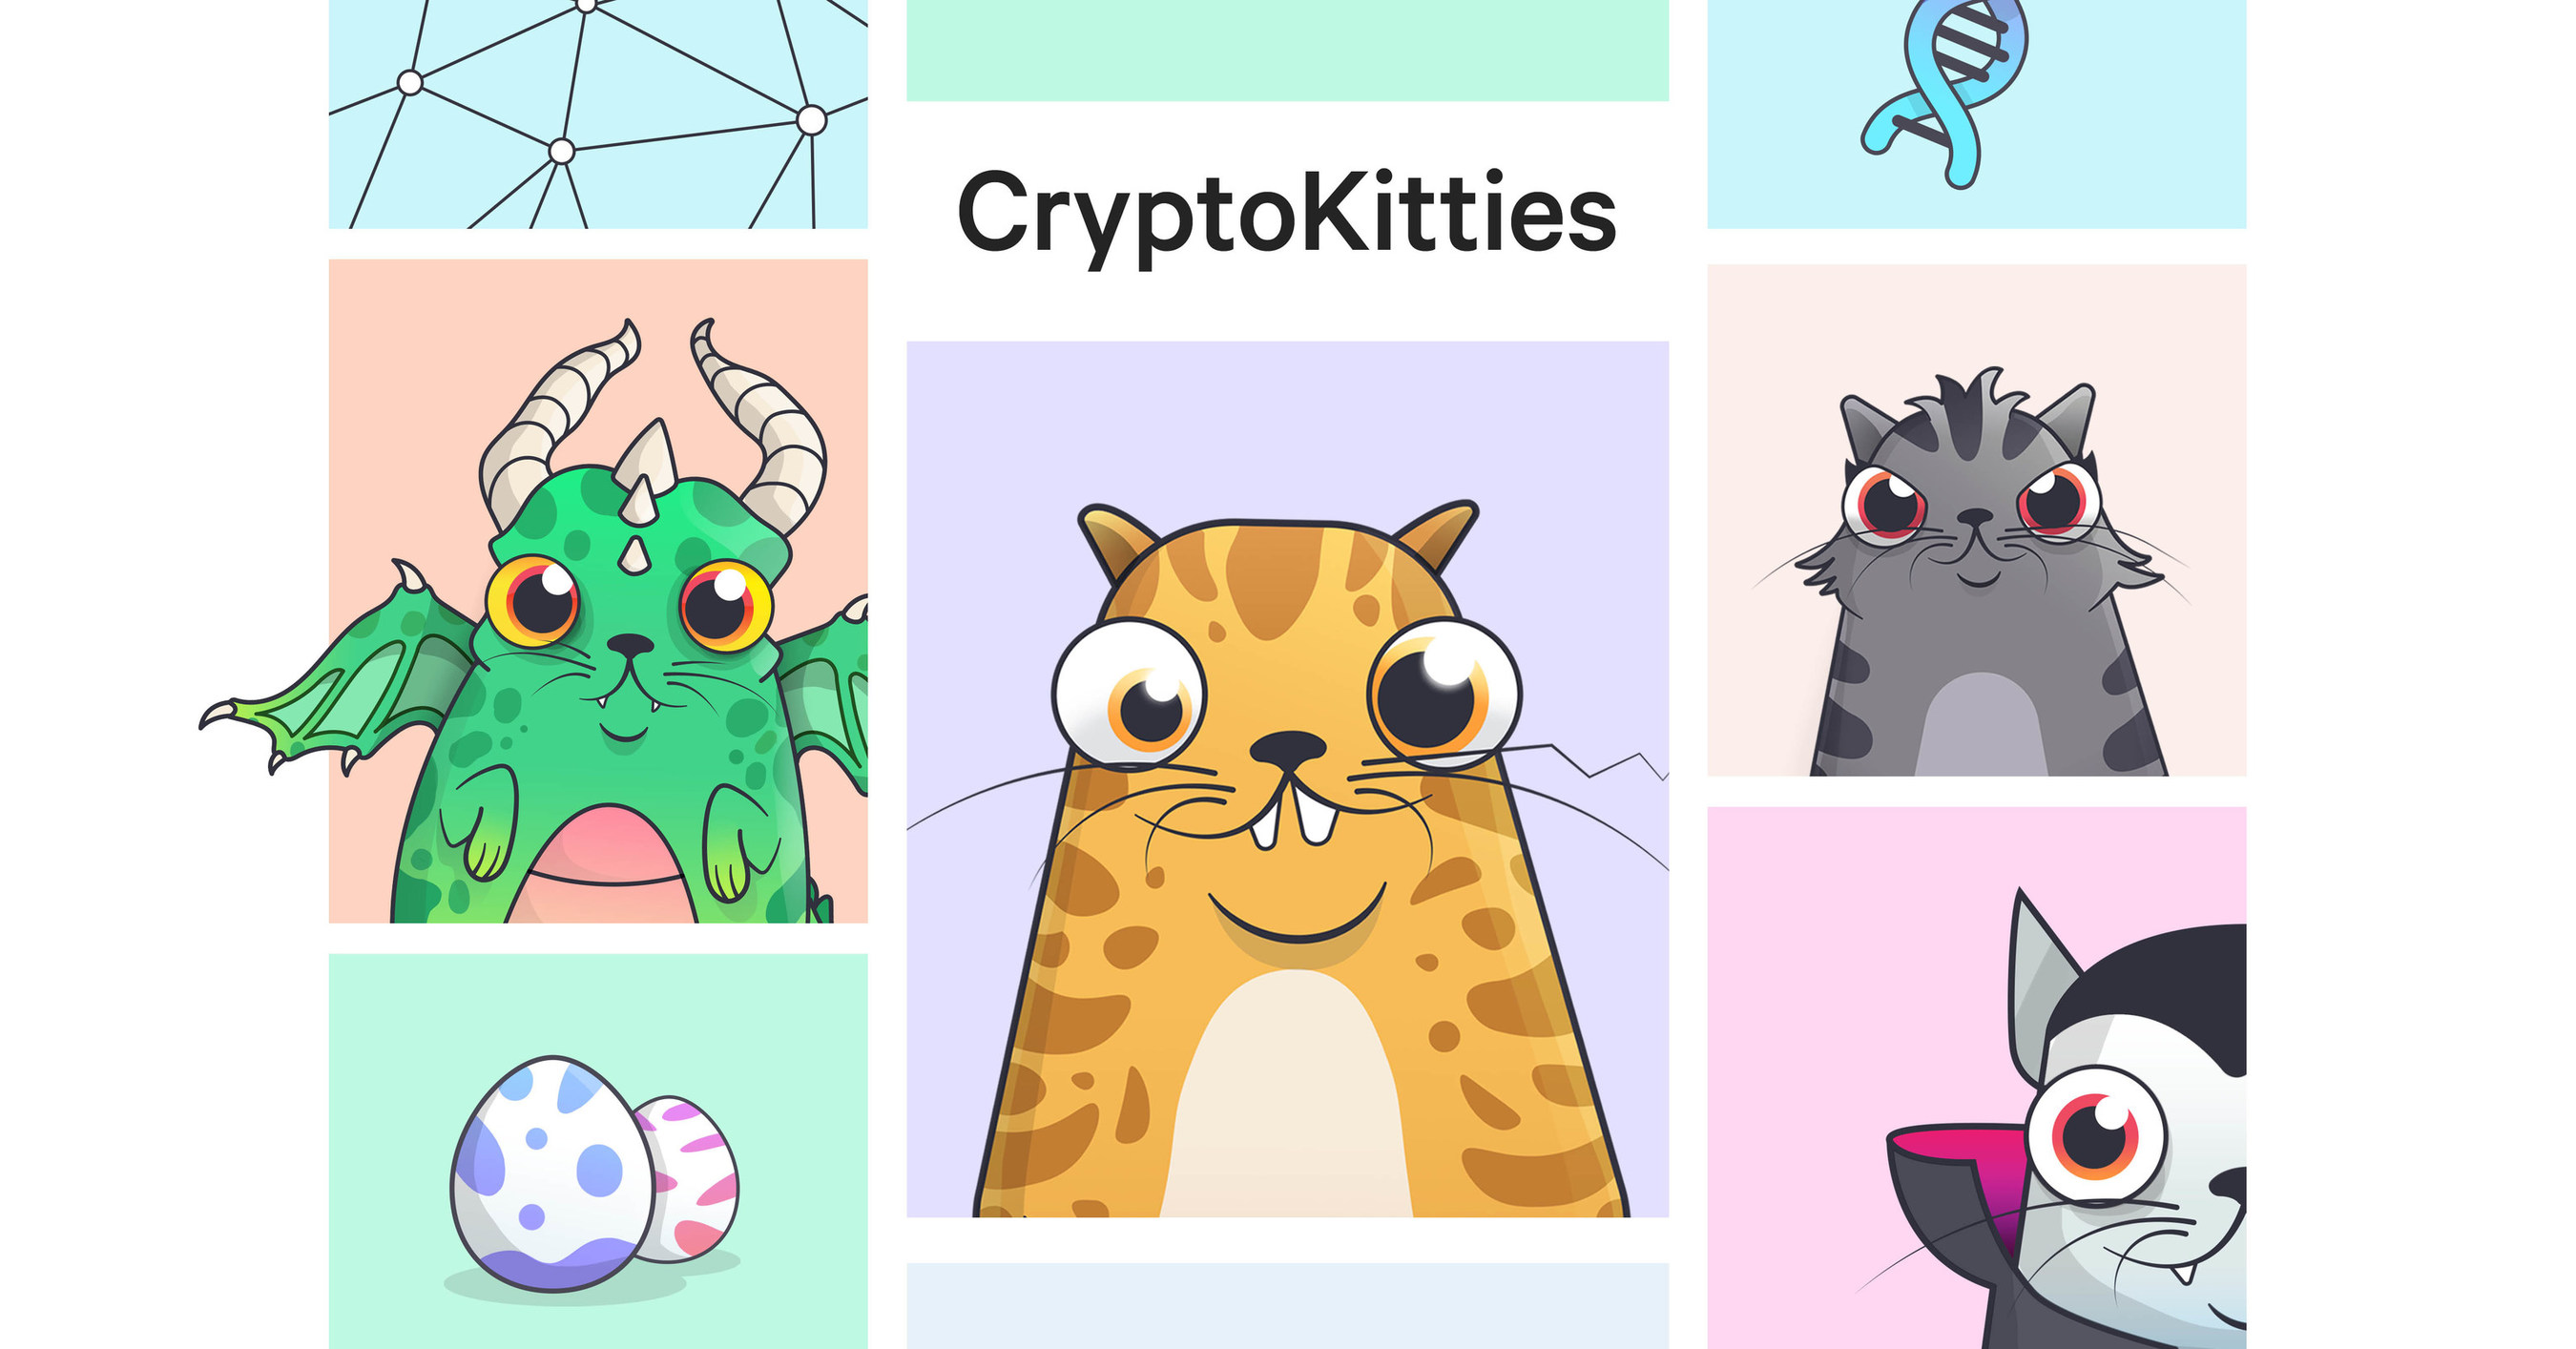
\includegraphics[scale = 0.3]{IMAGES/crypto_kitties.jpg}
    		\caption{Логотип децентралізованого додатку CryptoKitties.}
    		\label{fig:app_view_main_screen}
	\end{figure}

У загальних рисах можна додати, що CryptoKitties – це гра, де можна колекціонувати та розводити віртуальних котів. Кожен кіт є унікальним та представлений незамінним токеном (NFT) на блокчейні Ethereum. Тобто це означає, що кожен кіт є єдиним у своєму роді і його можна купити, продати або схрестити для отримання нових котів з цінними рисами. Ця гра була однією з перших, хто використовував технологію блокчейн, і допомогла популяризувати NFT. 

\begin{remark}
    \textbf{Чому децентралізовані додатки так важливі}?

    Децентралізовані програми (dApps) важливі, оскільки вони можуть суттєво змінити спосіб управління інформацією та ресурсами. На відміну від традиційних програм, dApps виключають посередників, що може знизити витрати та підвищити ефективність. Вони також використовують технологію блокчейн для підвищення безпеки, роблячи дані захищеними від підроблення. Також, dApps доступні будь-кому, хто має інтернет, що сприяє глобальному доступу до послуг, цифрових активів та інформації. Саме ця широка доступність і відкрита участь робить dApps такими революційними.
\end{remark}

Не дивлячись на плюси описаної платформи не можна не сказати про можливий скам, який дуже поширений серед них, а особливо фішингові атаки, що допомагають дізнатися особисті ключі користувача та здійснити атаку із можливим викраденням коштів. 

Далі не можна не підсумувати та навести плюси і мінуси даної архітектури для додатків.
\begin{itemize}
    \item \textbf{\textit{Плюси}}
        \begin{enumerate}
            \item \textbf{Зберігання особистої інформації відсутнє.} 
            
            Багато переваг dApps зосереджені навколо здатності програми захищати конфіденційність користувачів. У децентралізованих програмах користувачам не потрібно надавати свою особисту інформацію, щоб використовувати функції, які надає програма. DApps використовують розумні контракти для завершення транзакцій між двома анонімними сторонами без необхідності покладатися на центральний орган.
            
            \item \textbf{Неможливість блокування повідомлення.}
            
            Прихильники свободи слова зазначають, що dApps можна розробляти як альтернативні платформи соціальних мереж. Децентралізована платформа соціальних мереж стійка до цензури, оскільки жоден учасник блокчейну не може видаляти або блокувати повідомлення.
            
            \item \textbf{Простота створення нових децентралізовних додатків.}
            
            Ethereum — це гнучка платформа для створення нових dApps, яка забезпечує інфраструктуру, необхідну для розробників, щоб зосередити свої зусилля на пошуку інноваційних способів використання цифрових програм. Це може забезпечити швидке розгортання dApps у багатьох галузях, включаючи банківську справу та фінанси, ігри, соціальні мережі та онлайн-магазини.
        \end{enumerate}
    \item \textbf{\textit{Мінуси}}
        \begin{enumerate}
            \item \textbf{Все ще експериментальна технологія.}

            Використання dApps все ще знаходиться на ранніх стадіях, тому воно є експериментальним і схильне до певних проблем і невідомостей. Є питання щодо того, чи зможуть програми ефективно масштабуватися. Існують побоювання, що програма, яка потребує значних обчислень, перевантажить мережу, спричиняючи перевантаження мережі.
            
            \item \textbf{Складність переходу на Web3 додатки.}

            Здатність розробити зручний для користувача інтерфейс є ще однією проблемою. Більшість користувачів програм, розроблених традиційними централізованими установами, очікують простоти у використанні, що заохочує їх використовувати та взаємодіяти з програмою. Для того, щоб змусити людей перейти на dApps, від розробників потрібно створити умови для кінцевого користувача та рівень продуктивності, який конкуруватиме з популярними та визнаними програмами.
           
            \item \textbf{Складність модифікації уже опублікованих додатків.}

            Іншим обмеженням dApps є складність модифікації коду. Після розгортання dApp, імовірно, потребуватиме постійних змін, щоб удосконалити або виправити помилки чи ризики для безпеки. Відповідно до Ethereum, розробникам може бути складно внести необхідні оновлення в dApps, оскільки дані та код, що опубліковані у блокчейні, важко змінити.
        \end{enumerate}
\end{itemize}


\section{Відомі атаки}

Не дивлячись на використання децентралізованої мережі для запуску додатків всеодно існує ризик до взламу додатків. Розгляньмо одні із останніх, які спричинили мільйонні втрати.

\begin{itemize}

    \item \textbf{Вразливість Ronin мережі}

        Вразливість Ronin мережі була використана для масивної крадіжки криптовалюти, які взбудоражила всю індустрію. Сам взлом почався ще у листопаді 2021 року, коли база користувачів виросла до неймовірних розмірів. Компанії для подолання шаленого навантаження прийшлося збільшити очислювальні можливості та послабити процедури безпеки, щоб справитися із попитом. Трохи згодом, коли все стабілізувалося, то розробники не повернули процедури безпеки до початокового вигляду, тож цим і скористувалися зловмисники. Ця атака була проведена у грі \textit{Axie Infinity}, яка використовувала Ronin мережу. У результаті атаки було вкрадено 615 млн. доларів. 
    
    \item \textbf{Хак Cashio}
    
        У березні 2022 року базована на Solana Cashio стейбл коін CASH був жертвою хаку, який використовує вразливість "нескінченного випуску монет". Одразу після того CASH токен опустився на своє дно у ціні до 0.00005\$. Треба зазначити, що даний токен можна отримати лише за допомогою депозиту певної застави. Зловмисники використали недосконалу система валідації транзакцій. У даній ситуації можна було внести як депозит монети, які не були випущені певним існуючим банком. Тобто мережа не перевіряла існування певного банку настільки, що можна було вставити будь-яке значення. У результаті атаки було вкрадено 615 млн.\$.
    
    \item \textbf{Хак Exactly Protocol}
    
        Exactly Protocol -- DeFi проект, що заснований на блокчейні Optimism. Зловмисник скористався вразливістю в контрактах протоколу, щоб викрасти з проекту понад 7 мільйонів доларів. Злом Exactly Protocol є прикладом злому, активованого слабкими перевірками перевірки. Зловмисник зміг обійти перевірку дозволу на периферійний контракт DebtManager протоколу, надавши йому адресу підробленого шкідливого ринкового контракту. Після встановлення цього зловмисного контракту зловмисник виконав функцію зловмисного депозиту, яка надала доступ до коштів, які користувачі внесли в контракти протоколу. Загалом зловмисник зміг викрасти з проекту приблизно 7,3 млн \$ у ETH.
        
    \item \textbf{Хак Stake.com}

        Stake.com -- казино, яке використовує криптовалюти для приймання ставок. Інцидент Stake.com був спочатку виявлений на основі серії аномальних транзакцій на Ethereum. Зловмисник викрав близько 16 мільйонів доларів з рахунків казино Ethereum, а також 25,6 мільйонів \$, викрадених на BSC і Polygon. Атака включала лише підозрілі перекази з гарячих гаманців без взаємодії зі смарт-контрактами. Як наслідок, найімовірнішою причиною є зламані закриті ключі. Зловмисник — або зловмисник — із доступом до закритих ключів може перенести викрадену вартість з облікових записів казино.

    \item \textbf{Хак Woofi}

        WOOFi зазнав атаки маніпулювання цінами на свій контракт WOOFi Swap на основі Arbitrum. Зловмисник скористався помилками в синтетичному проактивному алгоритмі створення ринку (sPMM) проекту, щоб отримати приблизно 8,75 мільйонів \$ прибутку.

        WOOFi включає sPMM, який розроблений для імітації того, як виглядають книги ордерів (ціна, спред, глибина тощо) на централізованій біржі. sPMM має можливість змінювати ціну, надану оракулом, щоб захистити від падіння та допомогти збалансувати пул. 
        
        Зловмисник маніпулював цією функціональністю за допомогою експлойту flashloan. Вони запозичили приблизно 7,7 мільйона токенів WOO та продали їх у пул, що змусило sPMM скоригувати ціну токенів WOO майже до нуля (\$ 0,00000009). Резервна перевірка цін на токени, яка використовує Chainlink, не включала ціну токена WOO. Саме з такою нижчою ціною зловмисник зміг обміняти приблизно 10 мільйонів токенів WOO практично за безцінь. Повторивши цей процес тричі протягом 13 хвилин, зловмисник зміг отримати чистий прибуток у розмірі приблизно 8,75 мільйона доларів після того, як вони повернули свої флеш-кредити.
        
        За словами WOO, ця вразливість здебільшого існувала через розширення платформи, щоб включити ринок кредитування на блокчейні Arbitrum. Унікальне поєднання токена WOO та ринку кредитування WOO стало можливим для використання sPMM.
        
        Великі свопи на його платформі були швидко виявлені системою моніторингу транзакцій WOOFI; однак швидкість атаки дозволила хакеру викрасти значні обсяги криптовалюти з платформи. Контракт WOOFi Swap v2 було заморожено приблизно на два тижні, оскільки команда вносила зміни, щоб вирішити проблему.
\end{itemize}

\chapter{Чернетки до вимог безпеки децентралізованих додатків}

У підсумку до наведених атак та найчастіших вразливостей звичайних веб додатків можна сформувати таку собі чернетку для визначення безпеки децентралізованих додатків.

\begin{itemize}
    \item \textbf{Cryptographic Failures}
    
        Цей пукт відповідає за те, що додаток використовує чи заслабкі чи неправильно імплементовані криптографічні криптопримітиви. Цю проблему можна зустріти у багатьох атаках, що були здійснені на dApps

    \item \textbf{OWASP Smart Contract Top 10}
    
        Цей пункт відповідає за перевірку на вразливість смартконтрактів, що широко залучені до їх реалізації. У тому списку, скоріше наведені лише проблеми, які можуть виникнути лише із контрактами. Список доступний за \href{https://owasp.org/www-project-smart-contract-top-10/}{покликанням}.

    \item \textbf{Private key exposure}
    
        Цей пункт відповідає за розкриття особистих ключів для зловмисника. Особисто на мою думку, перед користуванням того чи іншого децентралізованого сервісу одразу треба при реєстрації коротко пояснювати людям яким є правильне застосування додатку та які дані, ключі є чутливими. Тобто таким чином буде збільшуватися обізнаність людей про децентралізовані додатки та зменшуватися кількість взламів додатків.

    \item \textbf{Validation errors}
    
        Під помилками у валідації маю на увазі, що дуже валивим нюансом перед релізом додатку є правильна перевірка вхідних даних перед їх обробкою бекендом. Тобто у dApps повинно буде дуже потужна валідація вхідних даних задля того, щоб не допускати різного роду атак, як то трапилося із Cashio.        
        
    \item \textbf{Unhandled protocol problems}
    
        У даному під unhandled protocol problems мається на увазі апробація протоколів у тестовому середовищі перед релізом. Насамперед цей крок, на мою думку, повинен зменшити кількість можливих атак, що будуть створені для даного додатку. Тобто повинно бути таке собі захищене середовище, до якого можна буде залучати хакерів чи звичайних розробників до перевірки безпеки та правильності роботи додатку.

\end{itemize}

